\documentclass{article}
\usepackage{graphicx}
\usepackage[margin=1.5cm]{geometry}
\usepackage{amsmath}

\begin{document}
\twocolumn

\title{Wednesday Warm Up: Electrostatics I and II}
\author{Prof. Jordan C. Hanson}

\maketitle

\section{Memory Bank}

\begin{itemize}
\item \textbf{Voltage:} Let the negative change in \textbf{voltage}, $\Delta V$, with respect to distance, be equal to the electric field:
\begin{equation}
E = - \frac{\Delta V}{\Delta x} ~\rightarrow~ \vec{E} = -\nabla V
\end{equation}
The relationship between \textbf{voltage} and change in potential energy is
\begin{equation}
\Delta U = q \Delta V
\end{equation}
\item \textbf{Couloumb voltage}: Let a charge with magnitude $q$ be separated by a displacement $\vec{r}$ from a \textit{test charge}.  The voltage generated by $q$ is 
\begin{equation}
V(r) = \frac{k q}{r}
\end{equation}
The constant $k$ is $k=8.988 \times 10^9$ N m$^2$ C$^{-1}$.
\end{itemize}

\section{Electrostatics I and II}

\begin{enumerate}
\item Consider Fig. \ref{fig:1}.  Which path requires positive work?
\begin{itemize}
\item A: P2 to P1
\item B: P1 to P3
\item C: P3 to P4
\item D: P4 to P2
\end{itemize}
\item Consider Fig. \ref{fig:1}.  Which path requires negative work?
\begin{itemize}
\item A: P2 to P1
\item B: P1 to P3
\item C: P3 to P4
\item D: P4 to P2
\end{itemize}
\item Consider Fig. \ref{fig:1}.  Which of the follow is true of the total work, $W$, done to move the charge around the closed path?
\begin{itemize}
\item A: $W > 0$
\item B: $W = 0$
\item C: $W < 0$
\item D: Undetermined
\end{itemize}
\item Recall that the definition of work is $W = \vec{F} \cdot \Delta \vec{x}$.  If the path is complex, we can express this as an \textit{integral}:
\begin{equation}
W = \int \vec{F} \cdot d\vec{r}
\end{equation}
(a) Insert the Coulomb force between a source charge $q$, and a test charge $Q$, separated by a distance $r$, for $\vec{F}$.  For $d\vec{r}$, assume a path starting at $r_i$ and ending at $r_f$.  Perform the integral\footnote{\textit{Hint: this is like integrating a power law.}} (b) Recall the work-energy theorem, which states that $W = \Delta KE$.  This implies that, if energy is conserved, $W = -\Delta U$, the change in potential energy.  Using the relationship between $\Delta U$ and $\Delta V$, show that the voltage difference created by a source charge at the origin ($r=0$) between $r_i$ and $r_f$ is
\begin{equation}
V = kq \left( \frac{1}{r_f} - \frac{1}{r_i} \right)
\end{equation}
(c) What happens if $r_i \to \infty$? \\ \vspace{2cm}
\item Prove that if the total work is zero around any closed path for a source charge at the origin, then the \textit{line integral} of the E-field around a closed path is always zero:
\begin{equation}
\oint \vec{E} \cdot d\vec{r} = 0
\end{equation}
This is one way of showing the electrostatic force to be \textit{conservative.}
\end{enumerate}

\begin{figure}
\centering
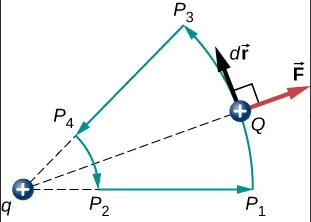
\includegraphics[width=0.25\textwidth,trim=0.05cm 0cm 0.1cm 0cm,clip=true]{figures/work.png}
\caption{\label{fig:1} Imagine moving a test charge $Q$ near a source charge $q$.  The four line segments form a \textit{closed path.}}
\end{figure}

\end{document}
